\documentclass[border=4pt]{standalone}
\usepackage{tikz}
\usetikzlibrary{positioning, arrows.meta, shapes.geometric, calc, fit, backgrounds}
\usepackage{amsmath,amssymb}
\begin{document}
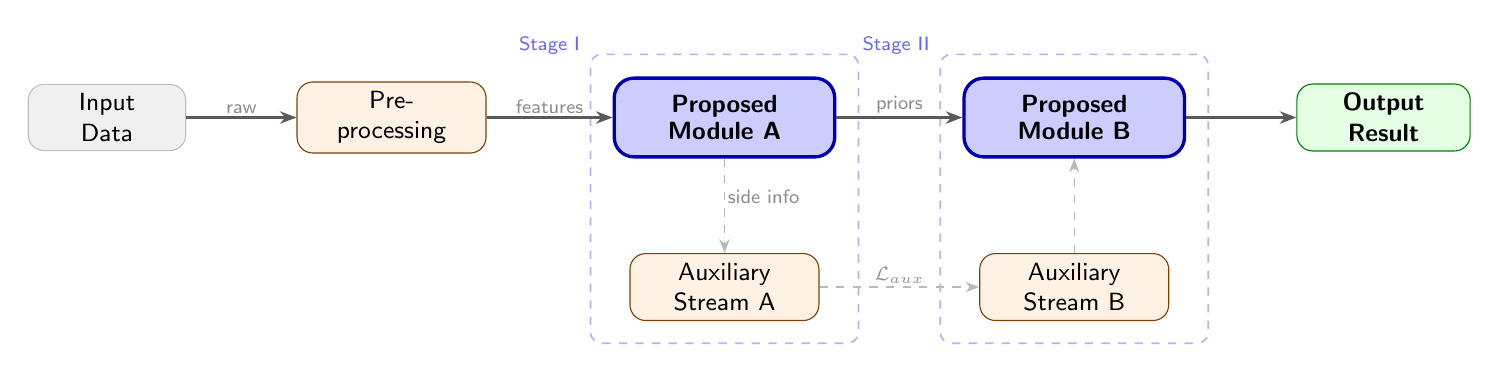
\begin{tikzpicture}[
  input/.style={draw, rounded corners=2mm, minimum width=2.0cm, minimum height=0.8cm,
                fill=gray!12, draw=gray!50, align=center, font=\sffamily\small},
  innov/.style={draw, rounded corners=2.5mm, minimum width=2.8cm, minimum height=1.0cm,
                fill=blue!20, draw=blue!70!black, line width=1.2pt, align=center,
                font=\sffamily\small\bfseries},
  proc/.style={draw, rounded corners=2mm, minimum width=2.4cm, minimum height=0.85cm,
               fill=orange!10, draw=orange!50!black, align=center,
               font=\sffamily\small},
  output/.style={draw, rounded corners=2mm, minimum width=2.2cm, minimum height=0.85cm,
                 fill=green!10, draw=green!50!black, align=center,
                 font=\sffamily\small\bfseries},
  arr/.style={-{Stealth[length=6pt]}, thick, color=black!65},
  arrd/.style={-{Stealth[length=5pt]}, dashed, color=gray!55},
  lbl/.style={font=\sffamily\scriptsize, text=black!45, fill=white, inner sep=1pt},
  gbox/.style={draw=blue!30, dashed, rounded corners=4pt, inner sep=8pt, line width=0.6pt},
]

% --- Row 1: Main pipeline ---
\node[input] (input) {Input\\Data};

\node[proc, right=1.4cm of input] (preproc) {Pre-\\processing};

\node[innov, right=1.6cm of preproc] (module1) {\textbf{Proposed}\\[-1pt]\textbf{Module A}};

\node[innov, right=1.6cm of module1] (module2) {\textbf{Proposed}\\[-1pt]\textbf{Module B}};

\node[output, right=1.4cm of module2] (output) {Output\\Result};

% --- Row 2: Auxiliary branch ---
\node[proc, below=1.2cm of module1] (aux1) {Auxiliary\\Stream A};
\node[proc, below=1.2cm of module2] (aux2) {Auxiliary\\Stream B};

% --- Main flow arrows ---
\draw[arr] (input) -- node[lbl, above] {raw} (preproc);
\draw[arr] (preproc) -- node[lbl, above] {features} (module1);
\draw[arr] (module1) -- node[lbl, above] {priors} (module2);
\draw[arr] (module2) -- (output);

% --- Auxiliary arrows ---
\draw[arrd] (module1) -- node[lbl, right, pos=0.4] {side info} (aux1);
\draw[arrd] (aux1) -- node[lbl, above] {$\mathcal{L}_{aux}$} (aux2);
\draw[arrd] (aux2) -- (module2);

% --- Grouping ---
\begin{scope}[on background layer]
  \node[gbox, fit=(module1)(aux1),
        label={[font=\sffamily\scriptsize, text=blue!60]above left:Stage I}] {};
  \node[gbox, fit=(module2)(aux2),
        label={[font=\sffamily\scriptsize, text=blue!60]above left:Stage II}] {};
\end{scope}

\end{tikzpicture}
\end{document}